\documentclass[crop,class=article]{standalone}
%----------------------------Preamble-------------------------------%
\usepackage{tikz}                       % Drawing/graphing tools.
\usetikzlibrary{arrows.meta}            % Latex and Stealth arrows.
\newcommand*\diff{\mathop{}\!\mathrm{d}}
%--------------------------Main Document----------------------------%
\begin{document}
    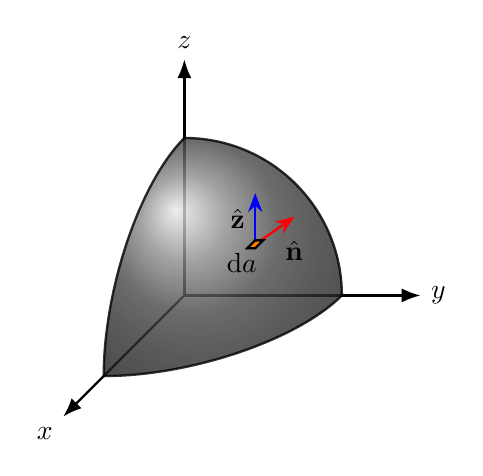
\begin{tikzpicture}[%
        line width=0.3mm,
        line cap = round,>={Latex},
        every edge/.style={draw=black,very thick}
    ]
        \draw[->] (0,0,0) -- (3,0,0) node[right] {$y$};
        \draw[->] (0,0,0) -- (0,3,0) node[above] {$z$};
        \draw[->] (0,0,0) -- (0,0,4) node[below left] {$x$};
        \draw[ball color=black!60!white,opacity=0.8]
            (2,0) arc (0:90:2) {[x={(0,0,1.33)}]
                  arc (90:0:2)} {[y={(0,0,1.33)}] arc (90:0:2)};
        \draw[->,>=Stealth,draw=blue] (0.9,0.65) --
            node [left] {$\hat{\mathbf{z}}$} (0.9,1.3);
        \draw[->,>=Stealth,draw=red] (0.9,0.65) --
            node [below right] {$\hat{\mathbf{n}}$} (1.4,1.0);
        \draw[fill=orange] 
            (0.8,0.6) to (0.9,0.6) to (1,0.7)
                      to (0.9,0.7) to cycle;
        \node at (0.73,0.67) [below] {$\diff{a}$};
    \end{tikzpicture}
\end{document}